\chapter{Lecture \thechapter{} of 18/03/2026}

\begin{theorem}[Charateodory, Book 1.2.1]

    Let $X \seq \Rn$ be nonempty. Then
    
    \begin{enumerate}
        \item[a)] every nonzero vector from $\cone{X}$ can be represented as a positive combination of linearly independent vectors in $X$;
        \item[b)] every vector fron $\conv{X}$ can be represented as a convex combination of no more then $n+1$ vectors in $X$.
    \end{enumerate}
    
\end{theorem}

\begin{proof}
    
    We prove a) and b) separately.

    \paragraph{a):} Let $y \in \cone{X} \implies y = \displaystyle\sum_{i=1}^m \alpha_i x_i$, where $\alpha_i > 0$, $x_i \in X$. We can assume $m$ to be the smallest index such that this representation holds true. We have to prove that $x_1,\dots,x_m$ to be linearly independent. By contraddiction, assume them dependent, so there exists $\lambda_1,\dots,\lambda_m \in \R$ such that $\displaystyle\sum_{i=1}^m \lambda_i x_i = 0$. Without loss of generality, assume at least one $\lambda_i > 0$. Define $\bar{\gamma} = \max\set{\gamma : \alpha_i -\gamma\lambda_i \ge 0} < +\infty$. Observe that we can write $y = \displaystyle\sum_i \alpha_i x_i + \bar{\gamma} \underbrace{\displaystyle\sum_i \lambda_i x_i}_{=0} = \displaystyle\sum_{i=1}^m (\alpha_i - \bar{\gamma}\lambda_i)x_i$. Then at leas one of the last coefficents is zero, which is in contraddiction with the minimality of $m$.

    \paragraph{b):} Consider the set $Y = \set{(y,1) : y \in X} \seq \Rnp$. Let $x \in \conv{X} \implies x = \displaystyle\sum_{i=1}^m \gamma_i x_i$, $\displaystyle\sum_i\gamma_i = 1$. The point $(x,1) \in \cone{Y} \implies \displaystyle\sum_i \gamma_i (x_i,1) = (x,1)$. By point a), $(x,1) = \displaystyle\sum_{i=1}^m \alpha_i(\tilde{x}_i,1)$, with $(\tilde{x}_i,1)$ linearly independent in $Y$. Hence $x = \displaystyle\sum_{i=1}^m \alpha_i \tilde{x}_i$ with $\displaystyle\sum_i \alpha_i = 1$. From the fact that $(\tilde{x}_i,1)$ are independent in $Y$, we conclude that $m \le n+1$.

\end{proof}

\begin{proposition}
    
    Let $X \seq \Rn$ be compact (closed and bounded). Then $\conv{X}$ is compact.

\end{proposition}

\begin{proof}
    
    It is easy to show that $\conv{X}$ is bounded. Since $X$ is bounded, $\exists R >0$ such that $\norm{x} \le R$ for any $x \in X$. Then $x \in \conv{X} \iff x = \displaystyle\sum_i \gamma_i x_i \implies \norm{x} \le \displaystyle\sum_i \gamma_i \norm{x_i} \le \displaystyle\sum_i \gamma_i R = R$.

    \paragraph{Closerness:} Take a sequence $\set{x_k^k}_k \seq \conv{X}$ and assume $x_k \to \bar{x}$ as $k \to +\infty$. We want to show that $\bar{x} \in \conv{X}$. Each $x^k$ can be written as

    \[ x_k = \displaystyle\sum_{i=1}^m \alpha_i^k x_i^k \]

    by the Charateodory's theorem, with $\displaystyle\sum_i\alpha_i = 1$, $\alpha_i \ge 0$, $x_i \in X$. Consider the sequence $\set{(\alpha_1^k,\dots,\alpha_{n+1}^n,x_1^k\dots,x_{n+1}^k)} \seq \R^{n+1+n(n+1)} = \R^{(n+1)^2}$. This is a bounded sequence and converges (up to subsequences by BW) to $(\alpha_1,\dots,\alpha_{n+1},x_1,\dots,x_{n+1})$. Observe that, since $\displaystyle\sum_i \alpha_i^k = 1 \implies \displaystyle\sum_i \alpha_i = 1,\,\alpha_i\ge 0$. Observe furthermore that all $x_i \in X$ by closerness of $X$, so $\displaystyle\sum_i \alpha_i^k x_i^k \to \displaystyle\sum_i \alpha_i x_i$, hence $\bar{x} = \displaystyle\sum_{i=1}^{n+1} \alpha_i x_i$, hence $\bar{x} \in \conv{X}$.

\end{proof}

\pagebreak
\textbf{Relative interiors}

If we consider a convex set in $\Rn$ which lives on an $m$-dimensional variety, with $m < n$ (as in \ref{fig:riex}), we get that the interior points of that convex sets forms the emptyset. 

\begin{figure}[ht!]
    \centering
    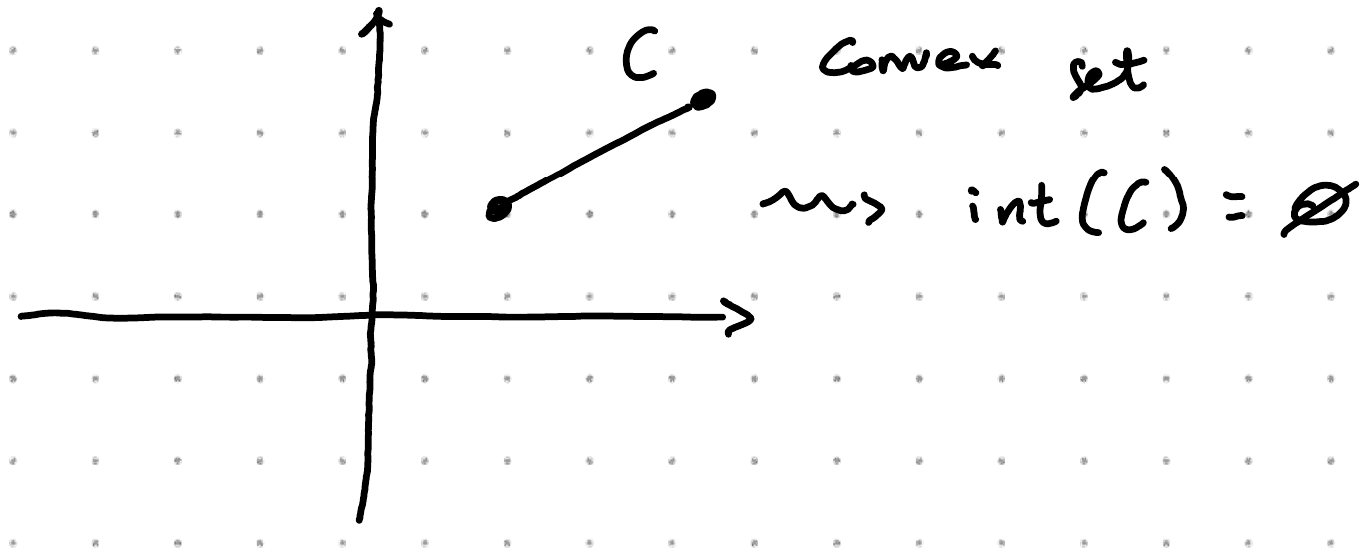
\includegraphics[width=0.7\textwidth]{img/riex.png}
    \caption{Example of emptyness of interior}
    \label{fig:riex}
\end{figure}

\begin{definition}[Relative interior point]
    
    Let $C \seq \Rn$ be a convex set, $c \in C$. We say that $x$ is a \emph{relative interior point} if there exists an $r > 0$ such that $B(x,r) \cap \aff{C} \seq C$. 

    The \emph{relative interior} is the set of all the relative interior points, and we denote it with $\ri{C}$.

    Furthermore we say that $C$ is \emph{relatively open} if $C = \ri{C}$.

\end{definition}

\begin{proposition}[Line-segment principle (LSP), Book 1.3.1]

    Let $C$ be a nonempty convex set. If $x \in \ri{C}$ and $\bar{x} \in \cl{C}$, then all points on the line segment connecting $x$ and $\bar{x}$, except possibly $\bar{x}$ belongs to $\ri{C}$.
    
\end{proposition}

\begin{proof}
    
    Assume $\bar{x} \in C \implies x \in \ri{C}$, so there exists $r > 0$ such that $B(x,r) \cap \aff{C} \seq C$. Let $\alpha \in (0,1)$ and set $x_\alpha = \alpha x + (1-\alpha)\bar{x}$. We have to prove that $x_\alpha \in \ri{C}$ for all $\alpha \in (0,1)$. 

    Consider $B(x_\alpha,\alpha r)$, we have to show that $B(x_\alpha, \alpha r) \cap \aff{C} \seq C$. Pick $y_\alpha \in B(x_\alpha, \alpha r) \cap \aff{C}$. Observing that $y_\alpha$ belongs both to $B(x_\alpha, \alpha r)$ and $\aff{C}$, in particular there exists $z_\alpha \in \Rn$, $\norm{z_\alpha} \le \alpha r$ such that $y_\alpha = x_\alpha + z_\alpha$, hence $y_\alpha = \alpha x + (1-\alpha)\bar{x} + z_\alpha = \alpha\underbrace{\left(x + \frac{z_\alpha}{\alpha}\right)}_{\in B(x,r)} + \underbrace{(1-\alpha)\bar{x}}_{\in C}$. 

    Observe that $x + \frac{z_\alpha}{\alpha} \in \aff{C}$. Indeed $x \in \aff{C}$. Consider $z_\alpha = y_\alpha - x_\alpha$, then $x_\alpha \in C \implies x_\alpha \in \aff{C}$, while $y_\alpha \in \aff{C}$. Putting all toghether, $z_\alpha \in$ parallel space to $\aff{C}$, so we remain in the affine space, as we are summing a point in the affine space and a point in the parallel subspace. Moreover $x + \frac{z_\alpha}{\alpha} \in B(x,r)$ as $\norm{\frac{z_\alpha}{\alpha}} \le \frac{\alpha r}{\alpha} = r$, hence $ x + \frac{z_\alpha}{\alpha} \in C$. 

    Consider now the case $\bar{x} \in \cl{C} \setminus C$. Then there exists a sequence $\set{x_k}_k$ such that $x_k \to \bar{x}$ and $x_k \in C$ for all $k$. Apply then the previous argument to all $x_k$. Define $x_{k,\alpha} = \alpha x + (1-\alpha)x_k \implies B(x_{k,\alpha},r\alpha) \cap \aff{C} \seq C$ for all $k$ and $\alpha \in (0,1)$. Then the sequence $x_{k,\alpha} \to x_\alpha = \alpha x + (1-\alpha)\bar{x}$. For $k$ large enough, $B\left(x_\alpha,\frac{\alpha r}{2}\right) \seq B(x_{k,\alpha},r\alpha)$. Take the intersection with the affine hull, hence $B\left(x_\alpha,\frac{\alpha r}{2}\right) \cap \aff{C} \seq B(x_{k,\alpha},r\alpha) \cap \aff{C}$, showing that $x_\alpha \in \ri{C}$.

\end{proof}
